

\begin{figure}[H]
\centering
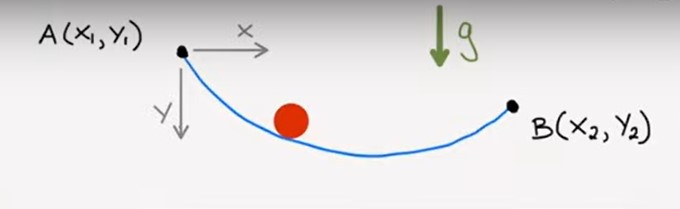
\includegraphics[width=13cm]{BrachPoints.jpg}
    		\caption{{A graphial representation of the Brachistochrone problem}}
\end{figure}

%\input{./}{BrachDia}


{The travel time between two points is the sum of the infinitesimal changes in the time taken to cover a fixed infinitesimal distance from the path length. If I, define the total time taken to be T, then the mathematical relation is defined as,}

	$$T = \int dt$$

{Because the phenomenon spans between in an finite time period, the above general integral can be written as,}

	$$T = \int_{t_{1}}^{t_{2}} dt$$

{Where, the phenomenon spans between $t = t_{1}$ and $t = t_{2}$. So, the solution to the problem is obtained when the optimization (minimization) of the time integral above is computed, ie. Obtaining the curve on which the optimization (minimization) of \textit{\textbf{T}} takes place.}

{If I define the velocity of the spherical mass in motion on the path (curve) to be,}

	$$v = \frac{ds}{dt}$$

{Where \textit{ds} is the incremental path length and \textit{dt} is the incremental time.}

{Implies,}

	$$dt = \frac{ds}{v}$$

{Making a substitution for \textit{dt} in the integral for \textit{\textbf{T}} yields,}

	$$T = \int \frac{ds}{v}$$

{Because this phenomenon consists of a finite path with a finite path length spanning between two points, namely $x_{1}$ and $x_{2}$, the above general integral can be written as,}

	\begin{equation}
		T = \int_{x_{1}}^{x_{2}} \frac{ds}{v}
		\label{T-ab}
	\end{equation}

{As I am considering \textit{y} to be the vertical distance (height) at an instant from point $x_{1}$ to the spherical mass on the curve, by the conservation of energy we have that the kinetic energy of the spherical mass at a point in time on curve is the loss in potential energy from height \textit{y}. Mathematically we have,}

	$$\frac{1}{2}mv^2 = mgy$$ 

{Implies,}

	$$v = \sqrt{2gy}$$

{If we look at the path (curve) closely and think about the infinitesimal path length \textit{ds}, in terms of \textit{dx} and \textit{dy}, we have by Pythagorean theorem,}

	$$ds^2 = dx^2 + dy^2$$

{Implies}

	$$ds = \sqrt{dx^2 + dy^2} = \sqrt{1 + \left(\frac{dy}{dx}\right)^2} dx = \sqrt{1 + \left(y^{\prime}\right)^2} dx$$

{Making a substitution for \textit{ds} and \textit{v} in equation \ref{T-ab}, we have,}

	$$T = \int_{x_1}^{x_2} \frac{ds}{v} = \int_{x_1}^{x_2} \frac{\sqrt{1 + \left(y^{\prime}\right)^2}}{\sqrt{2gy}} dx = \int_{x_1}^{x_2} \sqrt{\frac{1 + \left(y^{\prime}\right)^2}{2gy}} dx$$

{Therefore we have,}

	\begin{equation}
		T = \frac{1}{\sqrt{2g}}\int_{x_1}^{x_2} \sqrt{\frac{1 + \left(y^{\prime}\right)^2}{y}} dx
		\label{Tmin}
	\end{equation}

{Looking at the above equation, it is evident that conventional calculus methods do not apply here. Instead of the minimization of a specific point on a function, I have to minimize a family of curves (functions). This is because the function under the integral represents a category of special functions.}

\begin{figure}[H]
\centering
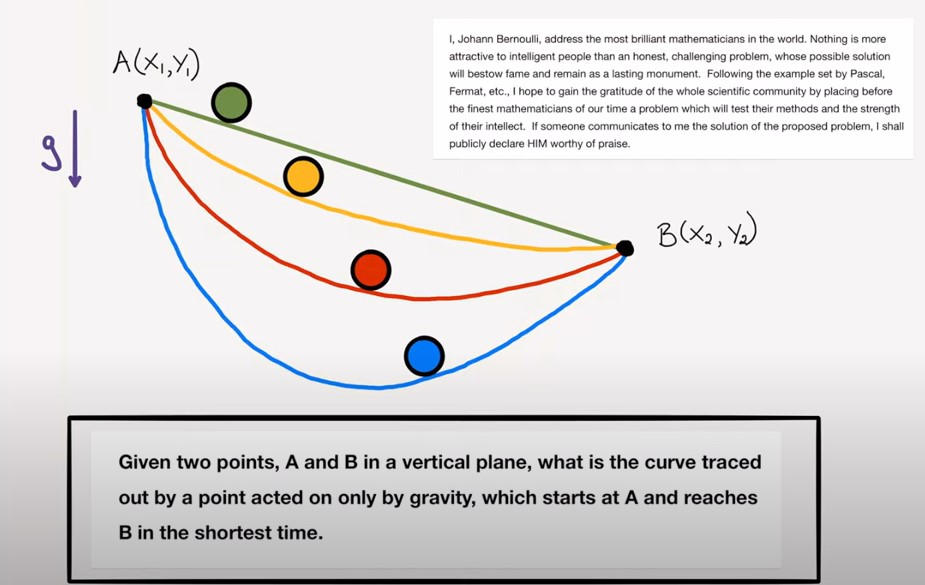
\includegraphics[width=13cm]{OrgProbDia.jpg}
    		\caption{{A graphial representation of some curves that could be a possible solution to the Brachistochrone problem}}
\end{figure}

{Upon observation we can evidently see that, $\sqrt{\frac{1 + \left(y^{\prime}\right)^2}{y}}$ is a special function in \textit{y} and \textit{$y^\prime$}. A function of this type (a function depending on a variable and their derivatives) is called a functional.}

{If we define this functional as \textit{F}, we have,}

	$$F[y,y^{\prime}] = \sqrt{\frac{1 + \left(y^{\prime}\right)^2}{y}}$$


